\documentclass[./../../paper.tex]{subfiles}
\graphicspath{{\subfix{./../../figures/}}}

\begin{document}

\section{Determine the Robustness given Sequence Length}
So far, the experiments were conducted on a maximal sequence length of \attention{25}. Also, we conducted each experiment\xixi{In terms of wording, should I change 'experiment' to 'simulation'?} on the same dataset. \attention{MENTION the RQ to have an approach which is \emph{process model agnositc}} With these result, we are not able to to claim, that thew model consistently outperforms the other approaches.  Therefore, this section will explore the results on different data-set sizes and types.


\subsection{Experimental Setup}
For this experiment, we run the same experiment of \autoref{sec:exp4} on all the datasets, that where introduced in \autoref{sec:dataset_description}.

\subsection{Results}
Again, \autoref{fig:exp5-winner} shows a clear dominance of the evolutionary model  (\attention{Model Name}) across all datasets. 

\begin{figure}[htbp]
    \centering
    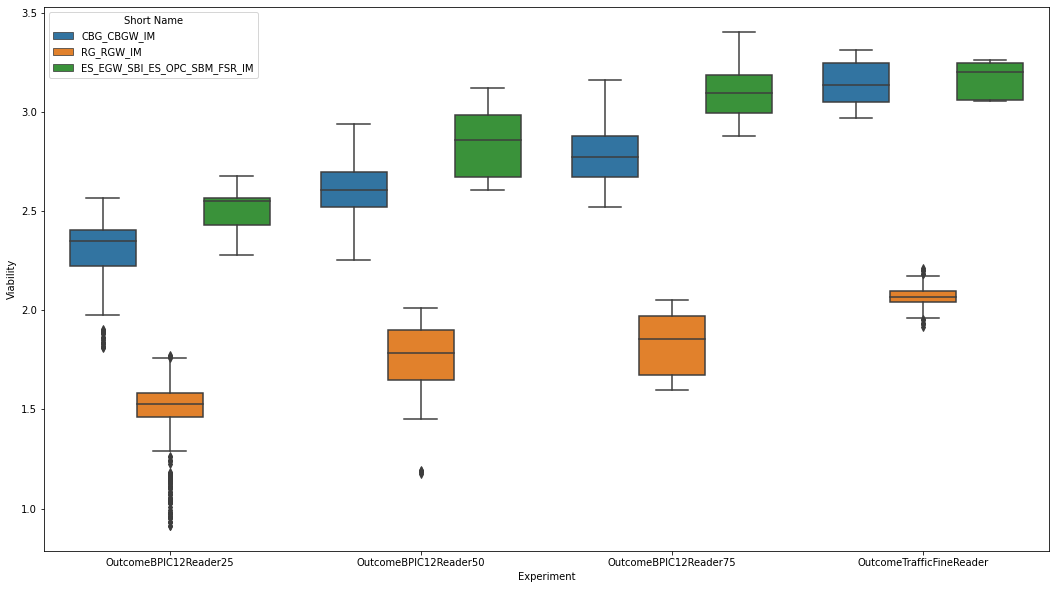
\includegraphics[width=\textwidth]{figures/generated/exp5_winner_overall.png}
    \caption{This figure shows boxplots of the viability of each models' generated counterfactual.}
    \label{fig:exp5-winner}
\end{figure}

The results show that the performance remains consistent for \attention{for a specific model}. Here, \attention{a specific model} returns an avarage viability of \attention{some value}. Hence, we can savely assume that the model outperforms the baseline approaches in general. 

However, a notable observation occurs in the processing time. Although all models require more time to produce their results, if we increase the maximum length of sequences, the evolutionary algorithms require substiantially more time. \autoref{tbl:exp5_duration} shows, the processing time is much higher than the baseline models. On average, \attention{evo model} require \attention{duration in seconds}, while \attention{other models} require \attention{XX}, \attention{XX} and \attention{XX}, respectively.

\subsection{Discussion}
The results show that \attention{... TBD}. The increase of generation time can be explained by the viability measure. More specifically, the current implementation of the \gls{SSDLD} within the sparsity and similarity measure have a quadratic time complexity. The time complexity primarily depends on the maximal sequence length. The number of cases that are compared is less of a factor as we use a highly vectorized implementation of the distance using numpy.   

\end{document}